\section{Faulted 3-phase network (2)}
\subsection{Type of fault}
From the waveforms presented in the assignment sheet, we see that as the fault occurs, the phase A and B voltages collapse, whilst the phase C voltage remains unaffected. The phase angle of A and B becomes the same and is \SI{180}{\degree} out of phase with respect to C. In terms of the current, we see that there is a significant increase in current magnitude in phase A and B. They are also \SI{180}{\degree} out of phase with each other. The unfaulted phase remains as is. We also see that there is no significant ground current in the faulted phases.

In terms of the standard fault sequence connections, the above can be summarised as:
\begin{align}
    V_a            & = V_b       \\
    \therefore V_1 & = V_2       \\
    I_a            & = -I_b      \\
    I_c            & \ll I_a     \\
    I_0            & = 0         \\
    \therefore I_c & = I_1 + I_2
\end{align}
where subscript $a$, $b$, $c$ represents phase and subscript $1$, $2$, $0$ represents positive, negative and zero sequence. Hence, the analysis is indicative of a line-to-line fault, occurring on phases A and B.
\subsection{Breaker circuit}
\begin{figure}[H]
    \centering
    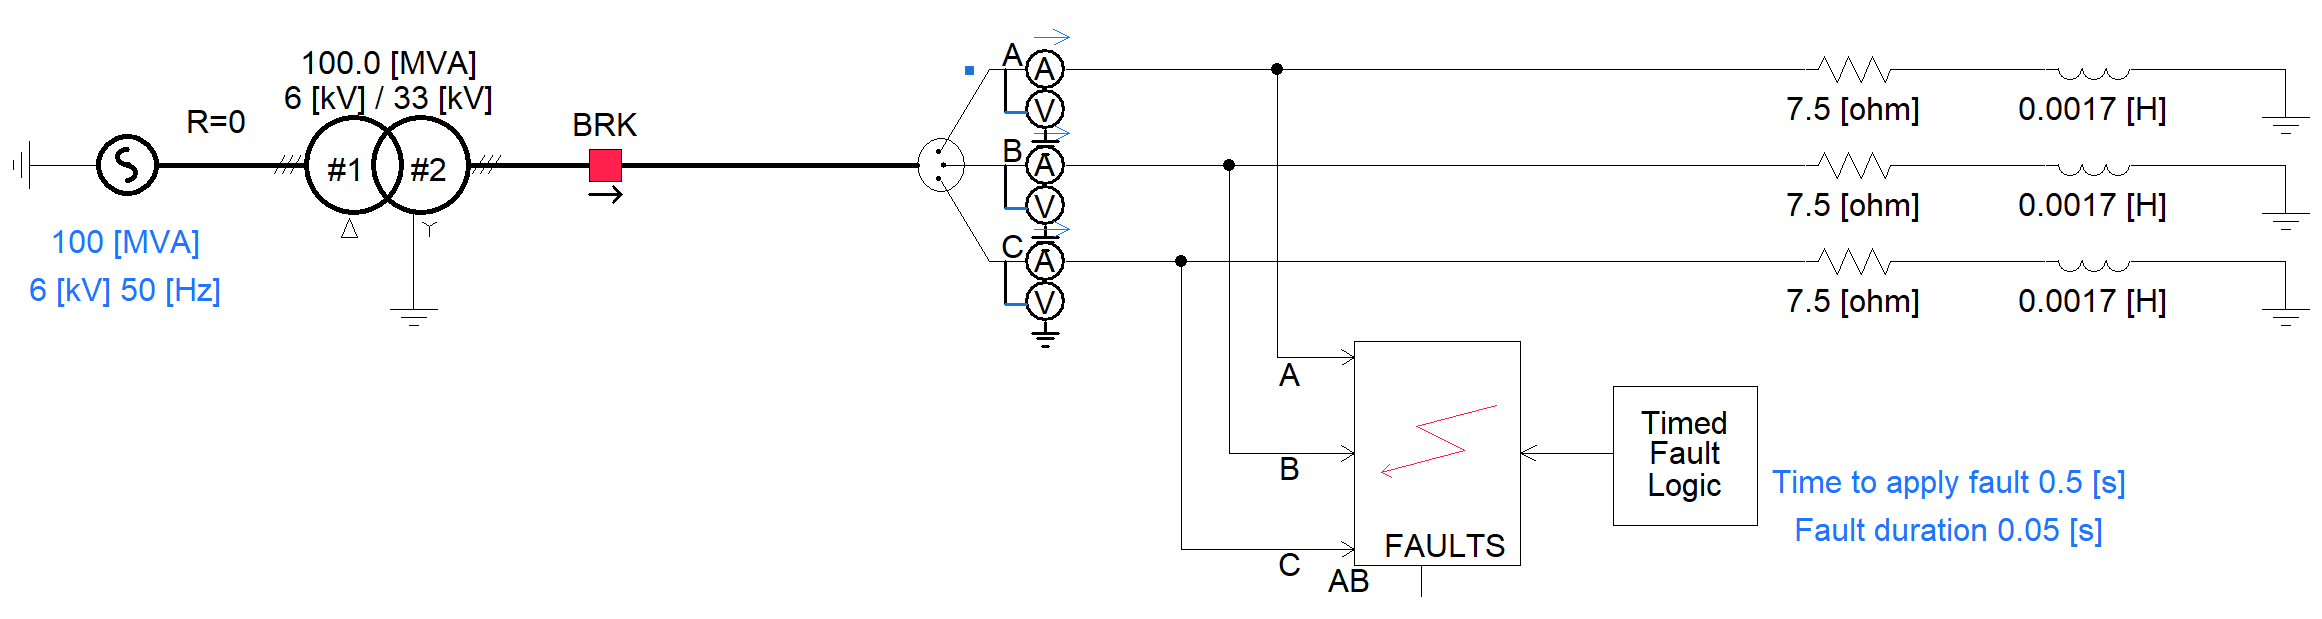
\includegraphics[width = \textwidth]{img/figure15.png}
    \caption{Circuit diagram to show distribution network with circuit breaker.}
    \label{fig:breakerNetwork}
\end{figure}
\begin{figure}[H]
    \centering
    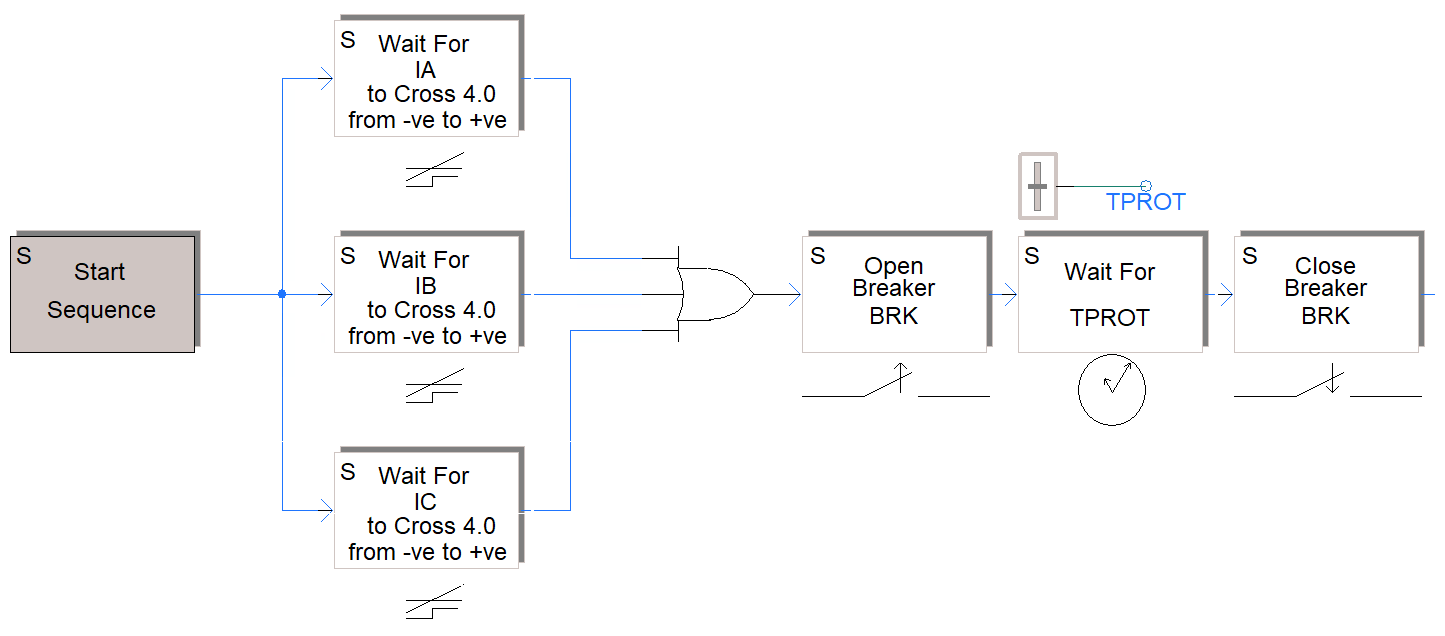
\includegraphics[width = \textwidth]{img/figure16.png}
    \caption{Sequencer diagram to show breaker activation logic.}
    \label{fig:sequencer}
\end{figure}
\begin{figure}[H]
    \centering
    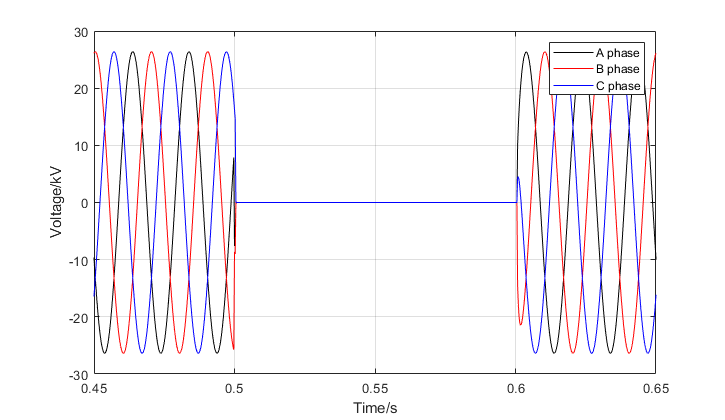
\includegraphics[width = \textwidth]{img/figure17.png}
    \caption{Faulted phase voltages over time from \SI{0.45}{\second} to \SI{0.65}{\second} with breaker circuit.}
    \label{fig:fault1BRK}
\end{figure}
\begin{figure}[H]
    \centering
    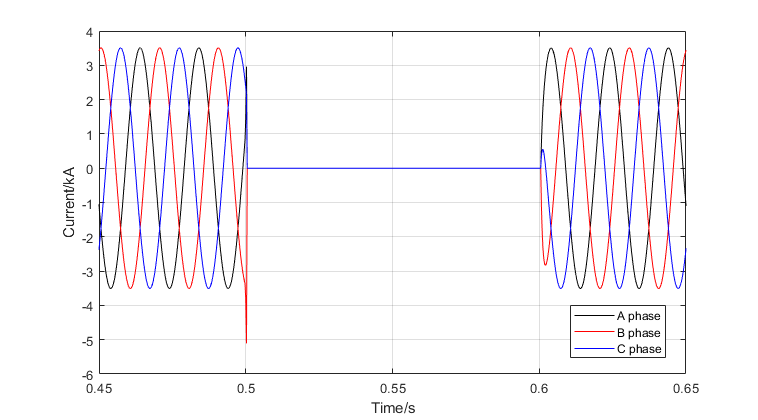
\includegraphics[width = \textwidth]{img/figure18.png}
    \caption{Faulted phase currents over time from \SI{0.45}{\second} to \SI{0.65}{\second} with breaker circuit.}
    \label{fig:fault2BRK}
\end{figure}
Using sequencer blocks within \textsc{PSCAD}, an approach where the breaker is tripped by measuring the fault current was chosen. A \textsc{Start Sequence} block is first, which then leads to three current measurement blocks. These operate on boolean principles, taking an initial value of 0 and flipping to a 1 when the programmed event occurs. In this case, the trip event is if the phase current exceeds the fault current. Note that in this design, the fault current can be changed to any value dependent on system requirements. A value of \SI{4}{\kilo\ampere} was chosen for testing purposes. The outputs of these blocks is inputted into an OR gate. A positive (`1') output from the OR gate triggers an \texttt{Open Breaker} block. The purpose of the OR gate is to activate the breaker in the case that any 1 phase displays fault current behaviour.

The function of \texttt{TPROT} is to simulate a manual delay of the breaker reactivation. In reality, fixing faults and reactivation of the circuit is a complex process. However, for the purposes of this simulation, a user can choose how long they would like their breaker to be open. Figure \ref{fig:fault2BRK} shows that the sequencer successfully trips the breaker when there is fault current (\texttt{TPROT} = \SI{1}{\second}).

MATLAB code may be viewed in Appendix \ref{app:q4}